\ifdefined\included
\else
\documentclass[a4paper,11pt,twoside]{StyleThese}
\usepackage{amsmath,amssymb}             % AMS Math
\usepackage[T1]{fontenc}
\usepackage[utf8x]{inputenc}
\usepackage{babel}
\usepackage{datetime}

\usepackage{lmodern}
\usepackage{tabularx}
%\usepackage{tabular}
\usepackage{multirow}

\usepackage{hhline}
\usepackage[left=1.5in,right=1.3in,top=1.1in,bottom=1.1in,includefoot,includehead,headheight=13.6pt]{geometry}
\renewcommand{\baselinestretch}{1.05}

% Table of contents for each chapter

\usepackage[nottoc, notlof, notlot]{tocbibind}
\usepackage{minitoc}
\setcounter{minitocdepth}{2}
\mtcindent=15pt
% Use \minitoc where to put a table of contents

\usepackage{aecompl}

% Glossary / list of abbreviations

\usepackage[intoc]{nomencl}
\iftoggle{ThesisInEnglish}{%
\renewcommand{\nomname}{Glossary}
}{ %
\renewcommand{\nomname}{Liste des Abréviations}
}

\makenomenclature

% My pdf code

\usepackage{ifpdf}

\ifpdf
  \usepackage[pdftex]{graphicx}
  \DeclareGraphicsExtensions{.jpg}
  \usepackage[a4paper,pagebackref,hyperindex=true]{hyperref}
  \usepackage{tikz}
  \usetikzlibrary{arrows,shapes,calc}
\else
  \usepackage{graphicx}
  \DeclareGraphicsExtensions{.ps,.eps}
  \usepackage[a4paper,dvipdfm,pagebackref,hyperindex=true]{hyperref}
\fi

\graphicspath{{.}{images/}}

%% nicer backref links. NOTE: The flag ThesisInEnglish is used to define the
% language in the back references. Read more about it in These.tex

\iftoggle{ThesisInEnglish}{%
\renewcommand*{\backref}[1]{}
\renewcommand*{\backrefalt}[4]{%
\ifcase #1 %
(Not cited.)%
\or
(Cited in page~#2.)%
\else
(Cited in pages~#2.)%
\fi}
\renewcommand*{\backrefsep}{, }
\renewcommand*{\backreftwosep}{ and~}
\renewcommand*{\backreflastsep}{ and~}
}{%
\renewcommand*{\backref}[1]{}
\renewcommand*{\backrefalt}[4]{%
\ifcase #1 %
(Non cité.)%
\or
(Cité en page~#2.)%
\else
(Cité en pages~#2.)%
\fi}
\renewcommand*{\backrefsep}{, }
\renewcommand*{\backreftwosep}{ et~}
\renewcommand*{\backreflastsep}{ et~}
}

% Links in pdf
\usepackage{color}
\definecolor{linkcol}{rgb}{0,0,0.4} 
\definecolor{citecol}{rgb}{0.5,0,0} 
\definecolor{linkcol}{rgb}{0,0,0} 
\definecolor{citecol}{rgb}{0,0,0}
% Change this to change the informations included in the pdf file

\hypersetup
{
bookmarksopen=true,
pdftitle="Évaluation de la sécurité des équipements grand public connectés à Internet",
pdfauthor="Yann BACHY", %auteur du document
pdfsubject="Thèse", %sujet du document
%pdftoolbar=false, %barre d'outils non visible
pdfmenubar=true, %barre de menu visible
pdfhighlight=/O, %effet d'un clic sur un lien hypertexte
colorlinks=true, %couleurs sur les liens hypertextes
pdfpagemode=None, %aucun mode de page
pdfpagelayout=SinglePage, %ouverture en simple page
pdffitwindow=true, %pages ouvertes entierement dans toute la fenetre
linkcolor=linkcol, %couleur des liens hypertextes internes
citecolor=citecol, %couleur des liens pour les citations
urlcolor=linkcol %couleur des liens pour les url
}

% definitions.
% -------------------

\setcounter{secnumdepth}{3}
\setcounter{tocdepth}{2}

% Some useful commands and shortcut for maths:  partial derivative and stuff

\newcommand{\pd}[2]{\frac{\partial #1}{\partial #2}}
\def\abs{\operatorname{abs}}
\def\argmax{\operatornamewithlimits{arg\,max}}
\def\argmin{\operatornamewithlimits{arg\,min}}
\def\diag{\operatorname{Diag}}
\newcommand{\eqRef}[1]{(\ref{#1})}

\usepackage{rotating}                    % Sideways of figures & tables
%\usepackage{bibunits}
%\usepackage[sectionbib]{chapterbib}          % Cross-reference package (Natural BiB)
%\usepackage{natbib}                  % Put References at the end of each chapter
                                         % Do not put 'sectionbib' option here.
                                         % Sectionbib option in 'natbib' will do.
\usepackage{fancyhdr}                    % Fancy Header and Footer

% \usepackage{txfonts}                     % Public Times New Roman text & math font
  
%%% Fancy Header %%%%%%%%%%%%%%%%%%%%%%%%%%%%%%%%%%%%%%%%%%%%%%%%%%%%%%%%%%%%%%%%%%
% Fancy Header Style Options

\pagestyle{fancy}                       % Sets fancy header and footer
\fancyfoot{}                            % Delete current footer settings

%\renewcommand{\chaptermark}[1]{         % Lower Case Chapter marker style
%  \markboth{\chaptername\ \thechapter.\ #1}}{}} %

%\renewcommand{\sectionmark}[1]{         % Lower case Section marker style
%  \markright{\thesection.\ #1}}         %

\fancyhead[LE,RO]{\bfseries\thepage}    % Page number (boldface) in left on even
% pages and right on odd pages
\fancyhead[RE]{\bfseries\nouppercase{\leftmark}}      % Chapter in the right on even pages
\fancyhead[LO]{\bfseries\nouppercase{\rightmark}}     % Section in the left on odd pages

\let\headruleORIG\headrule
\renewcommand{\headrule}{\color{black} \headruleORIG}
\renewcommand{\headrulewidth}{1.0pt}
\usepackage{colortbl}
\arrayrulecolor{black}

\fancypagestyle{plain}{
  \fancyhead{}
  \fancyfoot{}
  \renewcommand{\headrulewidth}{0pt}
}

%\usepackage{MyAlgorithm}
%\usepackage[noend]{MyAlgorithmic}
\usepackage[ED=MITT - STICRT, Ets=INSA]{tlsflyleaf}
%%% Clear Header %%%%%%%%%%%%%%%%%%%%%%%%%%%%%%%%%%%%%%%%%%%%%%%%%%%%%%%%%%%%%%%%%%
% Clear Header Style on the Last Empty Odd pages
\makeatletter

\def\cleardoublepage{\clearpage\if@twoside \ifodd\c@page\else%
  \hbox{}%
  \thispagestyle{empty}%              % Empty header styles
  \newpage%
  \if@twocolumn\hbox{}\newpage\fi\fi\fi}

\makeatother
 
%%%%%%%%%%%%%%%%%%%%%%%%%%%%%%%%%%%%%%%%%%%%%%%%%%%%%%%%%%%%%%%%%%%%%%%%%%%%%%% 
% Prints your review date and 'Draft Version' (From Josullvn, CS, CMU)
\newcommand{\reviewtimetoday}[2]{\special{!userdict begin
    /bop-hook{gsave 20 710 translate 45 rotate 0.8 setgray
      /Times-Roman findfont 12 scalefont setfont 0 0   moveto (#1) show
      0 -12 moveto (#2) show grestore}def end}}
% You can turn on or off this option.
% \reviewtimetoday{\today}{Draft Version}
%%%%%%%%%%%%%%%%%%%%%%%%%%%%%%%%%%%%%%%%%%%%%%%%%%%%%%%%%%%%%%%%%%%%%%%%%%%%%%% 

\newenvironment{maxime}[1]
{
\vspace*{0cm}
\hfill
\begin{minipage}{0.5\textwidth}%
%\rule[0.5ex]{\textwidth}{0.1mm}\\%
\hrulefill $\:$ {\bf #1}\\
%\vspace*{-0.25cm}
\it 
}%
{%

\hrulefill
\vspace*{0.5cm}%
\end{minipage}
}

\let\minitocORIG\minitoc
\renewcommand{\minitoc}{\minitocORIG \vspace{1.5em}}

\usepackage{multirow}
%\usepackage{slashbox}

\newenvironment{bulletList}%
{ \begin{list}%
	{$\bullet$}%
	{\setlength{\labelwidth}{25pt}%
	 \setlength{\leftmargin}{30pt}%
	 \setlength{\itemsep}{\parsep}}}%
{ \end{list} }

\newtheorem{definition}{Définition}
\renewcommand{\epsilon}{\varepsilon}

% centered page environment

\newenvironment{vcenterpage}
{\newpage\vspace*{\fill}\thispagestyle{empty}\renewcommand{\headrulewidth}{0pt}}
{\vspace*{\fill}}

\usepackage{tablefootnote}

\usepackage{hyperref}
\hypersetup{
     colorlinks   = true,
     citecolor    = violet
}
\usepackage{graphicx} % for pdf, bitmapped graphics files
\usepackage{amsmath} % assumes amsmath package installed
\usepackage{amssymb}  % assumes amsmath package installed
\usepackage{bm} % for using bold lowercase greek letters
\usepackage{array}
\usepackage{colortbl}	% to color table background
%\usepackage[table]{xcolor}
\usepackage{subfigure}  
\usepackage{tikz}
\newcommand{\tikzcircle}[2][red,fill=red]{\tikz[baseline=-0.5ex]\draw[#1,radius=#2] (0,0) circle ;}%
\definecolor{turquoise}{rgb}{0.28 1 0.92}
\newcommand{\fratop}[2]{\genfrac{}{}{0pt}{}{#1}{#2}}
\newcommand{\mx}[1]{\mathbf{\bm{#1}}} 				% Matrix symbol
\newcommand{\vc}[1]{\mathbf{\bm{#1}}} 					% Vector symbol
\newcommand{\degree}{\ensuremath{^\circ}}				% define the degree symbol
\newcommand{\pder}[2]{\frac{\partial#1}{\partial#2}}		% partial derivative
\newcommand{\ppder}[2]{\frac{\partial^2 #1}{\partial#2^2}}		% second partial derivative
\newcommand{\refframe}[1]{\mbox{\textless#1\textgreater}}	% to denote a reference frame
%\DeclareMathOperator*{\lexmin}{\text{lex}\!\min}			% lexmin
\DeclareMathOperator*{\minimize}{minimize}				% minimize
\DeclareMathOperator*{\maximize}{maximize}				% maximize
%\DeclareMathOperator*{\argmin}{\arg\!\min}				% argmin
%\DeclareMathOperator*{\argmax}{\arg\!\max}				% argmax
\DeclareMathOperator*{\st}{subject\,to}					% subject to
\DeclareMathOperator*{\dif}{\mathrm{d}}					% d
\DeclareMathOperator*{\half}{\frac{1}{2}}					% one half
\newcommand{\mat}[1]{\ensuremath{\begin{bmatrix}#1\end{bmatrix}}}	% matrix
\newcommand{\rank}[1]{\text{rank}(#1)}							% rank
%\newcommand{\diag}[1]{\text{diag}(#1)}							% diag
\newcommand{\x}{\ensuremath{\times}}
\newcommand{\spac}{\ensuremath{\quad}}						% alias for space in math environment
\newcommand{\dt}[0]{\ensuremath{\Delta t}}					% dt
\newcommand{\dx}[0]{\ensuremath{\delta x}}					% dx
\newcommand{\du}[0]{\ensuremath{\delta u}}					% du
\newcommand{\dhu}[0]{\ensuremath{\delta \hat{u}}}					% \hat{du}
\newcommand{\dbu}[0]{\ensuremath{\delta \bar{u}}}					% \bar{du}
\newcommand{\dtu}[0]{\ensuremath{\delta \tilde{u}}}					% \tilde{du}
\newcommand{\dhx}[0]{\ensuremath{\delta \hat{x}}}					% \hat{dx}
\newcommand{\DX}[0]{\ensuremath{\Delta X}}						% DX
\newcommand{\DU}[0]{\ensuremath{\Delta U}}						% DU
\newcommand{\Ts}[0]{\ensuremath{\top}}							% transpose symbol
\newcommand{\pinv}[0]{\ensuremath{\dagger}}					% pseudoinverse symbol
\newcommand{\Rv}[1]{\ensuremath{\mathbb{R}^{#1}}}				% set of real-valued vectors
\newcommand{\Rm}[2]{\ensuremath{\mathbb{R}^{#1\times #2}}}		% set of real-valued matrices
\newcommand{\Spd}[1]{\ensuremath{\mathbb{S}_+^{#1}}}			% set of symmetric positive-definite matrices
\newcommand{\card}[1]{\ensuremath{\left\vert{#1}\right\vert}}			% cardinality of a set
\DeclareMathOperator{\Tr}{Tr}							% trace
\newcommand{\Expect}{{\rm I\kern-.3em E}}				% expectation
\newcommand{\Normal}{\mathcal{N}}					% normal distribution
\newcommand{\Prob}[1]{\text{P}(#1)}						% probability
\newcommand{\vech}[1]{\text{vech}(#1)}						% vech

\newcommand{\sethree}{\ensuremath{SE(3)}}
\newcommand{\CS}{$\mathcal{CS}$}
\newcommand{\WS}{$\mathcal{WS}$}
\newcommand{\CSfree}{$\mathcal{CS}_{free}$}
\newcommand{\CSobst}{$\mathcal{CS}_{obst}$}
\newcommand{\M}[0]{$\mathcal{M}$}

%\algnewcommand{\algorithmicgoto}{\textbf{go to}}%
%%\algnewcommand{\Goto}[1]{\algorithmicgoto~\ref{#1}}%
%\algnewcommand{\Goto}{\algorithmicgoto\xspace}%
%\algnewcommand{\Label}{\State\unskip}

\newenvironment{definition}[1][Definition]{\begin{trivlist}
\item[\hskip \labelsep {\bfseries #1}]}{\end{trivlist}}

\usepackage{epstopdf}
\usepackage[colorinlistoftodos,prependcaption,textsize=tiny]{todonotes}
\newcommand\explainmore[1]{\textcolor{red}{#1}}
\newcommand\refrephrase[1]{\textcolor{yellow}{#1}}
\newcommand\donerephrasing[1]{\textcolor{green}{#1}}

%DIF PREAMBLE EXTENSION ADDED BY LATEXDIFF
%DIF UNDERLINE PREAMBLE %DIF PREAMBLE
\RequirePackage[normalem]{ulem} %DIF PREAMBLE
\RequirePackage{color}\definecolor{RED}{rgb}{1,0,0}\definecolor{BLUE}{rgb}{0,0,1} %DIF PREAMBLE
\providecommand{\DIFadd}[1]{{\protect\color{blue}\uwave{#1}}} %DIF PREAMBLE
\providecommand{\DIFdel}[1]{{\protect\color{red}\sout{#1}}}                      %DIF PREAMBLE
%DIF SAFE PREAMBLE %DIF PREAMBLE
\providecommand{\DIFaddbegin}{} %DIF PREAMBLE
\providecommand{\DIFaddend}{} %DIF PREAMBLE
\providecommand{\DIFdelbegin}{} %DIF PREAMBLE
\providecommand{\DIFdelend}{} %DIF PREAMBLE
%DIF FLOATSAFE PREAMBLE %DIF PREAMBLE
\providecommand{\DIFaddFL}[1]{\DIFadd{#1}} %DIF PREAMBLE
\providecommand{\DIFdelFL}[1]{\DIFdel{#1}} %DIF PREAMBLE
\providecommand{\DIFaddbeginFL}{} %DIF PREAMBLE
\providecommand{\DIFaddendFL}{} %DIF PREAMBLE
\providecommand{\DIFdelbeginFL}{} %DIF PREAMBLE
\providecommand{\DIFdelendFL}{} %DIF PREAMBLE
%DIF END PREAMBLE EXTENSION ADDED BY LATEXDIFF


\begin{document}


\sloppy
\begin{document}
\setcounter{chapter}{2}
\fi

\chapter*{Conclusion}
\addstarredchapter{Conclusion} %Sinon cela n'apparait pas dans la table des matières
It is very clear robustness in robotic control is quite an essential aspect that has been given less importance in experimental robotics. Both the contributions addressed the issues of handling uncertainties and variability in robotic control in different platform and in different settings. This thesis illustrates the application of the contributed strategies in both industrial and humanoid robots to avoid robot and task failures. 
\section{Dynamic Obstacle Avoidance}
The first contribution is a framework that augments robot manipulators with dynamic obstacle avoidance functionality to become collaborative with human beings. The framework uses proximity skin sensors to sense the distance between the local sensor positions on the arm and the obstacles. The dense proximity information around the arm gives way to be reactive in robot's workspace. The kinect based reactive planner along with the reactive controller allows to handle obstacles dynamically with  point cloud and proximity information. These heterogenous components are integrated within ROS middleware framework to establish control in Universal Robot UR5. The preliminary tests are conducted in simulation and there is an ongoing effort to demonstrate the dynamic obstacle avoidance behavior in a real robot setup shown in Fig.\ref{fig:TUDSetup}. 


The reactive controller uses the state of the art hierarchical QP based optimization solver which makes it efficient to be used in real time. The tasks are programmed systematically to execute the planned trajectory while it avoids the potential collisions either by the virtue of the higher priority collision avoidance task or replan a new trajectory when the robot hits a local minima. 


The integration and installation of advanced functionalities such as the dynamic
obstacle avoidance solution presented poses three main challenges from the
software point of view. The first is the integration of different components such as the skin driver, path planner and robot motion control. We address this challenge by adhering to the software development paradigm of the ROS-Industrial initiative. All the components discussed in this paper have been successfully integrated with ROS.

A second challenge is the quality assurance and robustness of the integrated robot software. This is crucial in production environments, and is specially important in collaborative applications, where safety needs to be guaranteed. For this purpose an Automated testing Framework (ATF) has been developed \cite{Weisshardt-2016} as a part of the FiaD prohect, which
allows for the systematic testing of robot software components, which includes unit
 testing, simulation-in-the-loop testing and eventually hardware-in-the-loop testing.
The tests can be automated and integrated in a centralized continuous
integration system. Preliminary test have already been conducted with the
components of the robot software system of this work, and the integrated
prototype applications will be tested with ATF.

Finally, the third challenge is the deployment of the software. One of the main barriers to transfer solutions based on robot frameworks such as ROS to industry, and specially SMEs, is how cumbersome it is
to deploy. As a part of the FiaD project, a Robot deployment toolbox has been developed \cite{Ludtke-2017}, based on ROS, which can also be integrated with ATF. The deployment tools will also be evaluated on the RBE17 prototype.

\begin{figure*}[!h]
\centering
\begin{subfigure}
[PR2 Robot]{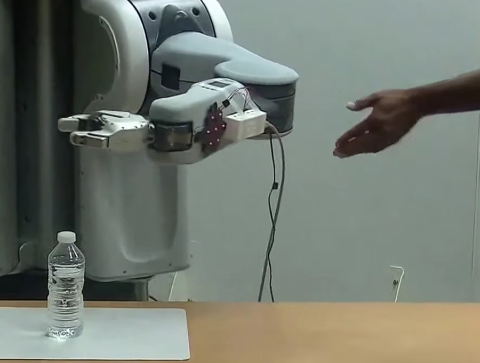
\includegraphics[width=5.5cm,height=6cm]{doa/images/pr2_1.png}}
\end{subfigure}\quad
\begin{subfigure}
[TOMM Setup]{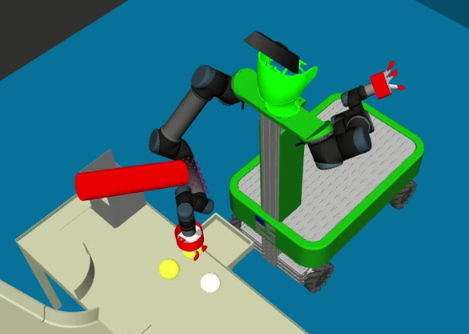
\includegraphics[width=5.5cm,height=6cm]{doa/images/tomm_replan.png}}\quad
\end{subfigure}
\caption{Preliminary tests done in simulation and robot}
\label{fig:conclusion_tests}
\end{figure*}
% \begin{figure*}[!h]
% \centering
% {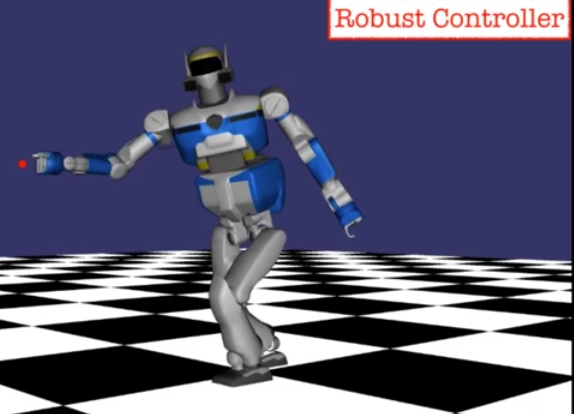
\includegraphics[scale=0.5]{rc_inertial_params/final.png}}
% \caption{Robust Control}
% \label{fig:robc}
% \end{figure*}



\section{Robust Controller}
The second contribution is a strategy to model inertial uncertainties indirectly in the capture-point inequality constraint within the Task Space Inverse Dynamics framework. The capture-point constraint takes care of the balancing in this framework and modeling uncertainties in this constraint makes the controller robust to inertial errors of the robot model.  

\begin{figure*}[!h]
\centering
\begin{subfigure}
[Classic Controller]{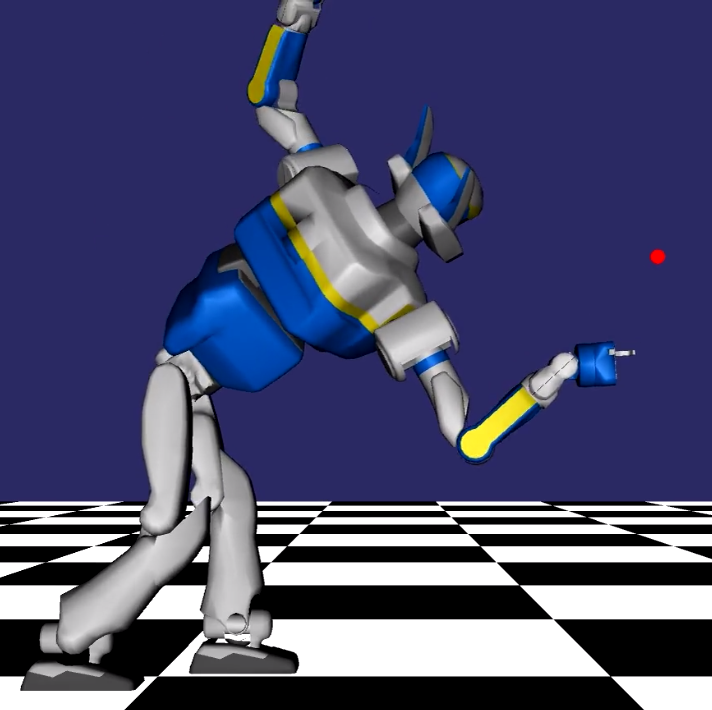
\includegraphics[scale=0.22]{rc_inertial_params/classic.png}}
\end{subfigure}\quad
\begin{subfigure}
[Robust Controller]{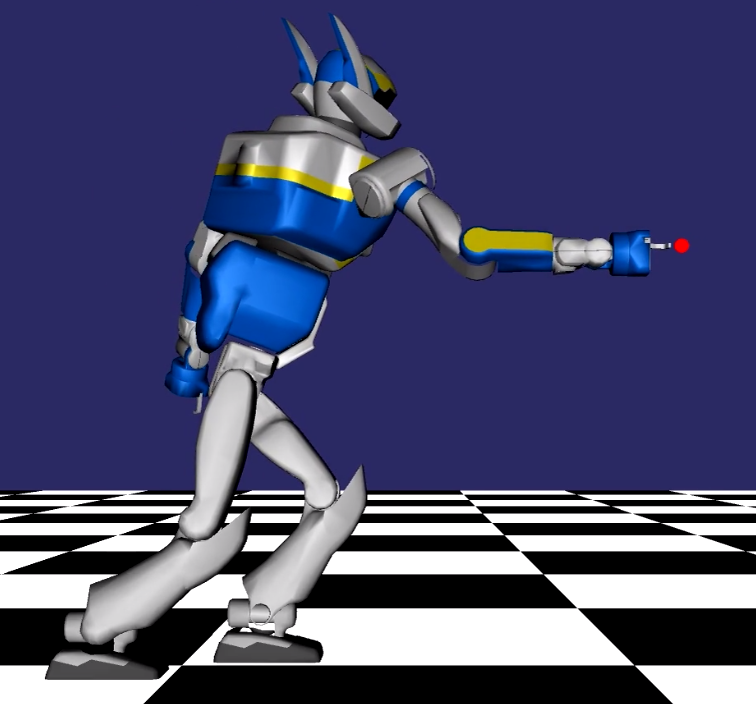
\includegraphics[scale=0.22]{rc_inertial_params/robust.png}}
\end{subfigure}\quad
\caption{Reaching Task under Inertial Uncertainties}
\label{fig:robc}
\end{figure*}

In the derivation of the robust controller we saw that the inertial parameters appear in different terms of the optimization problem.
In this preliminary work we focused only on how the uncertainties affect the CoM position.
We believe it should be possible to extend this analysis to the other terms in the capture-point inequalities: CoM velocity, CoM altitude, CoM Jacobian and its time derivative. 
Extending it also to the mass matrix and the bias forces is an interesting future direction, but it seems more challenging because of nonlinearities.

Another issue of the presented approach is that it is rather conservative and this can lead to poor performance, which can be unacceptable on a real system. Modeling uncertainties with probability distributions (rather than with polytopes) may lead to a less conservative behavior of the system, and it is thus an interesting future direction. In ~\cite{DelPrete2015b}, the proposed controller was robust to joint-torque tracking errors. Integrating the two controllers together seems to be feasible and it would provide robustness to both kinds of uncertainties. In this preliminary work we focused on simulations to validate the controller formulation and to test it with different parameter errors. Of course, we plan also to test the generated movements on the real HRP-2 robot, to quantify how much it can benefit from this robustness.



\ifdefined\included
\else
\bibliographystyle{acm}
\bibliography{These}
\end{document}
\fi